\section{Opcional 1. Càlcul de $S$ i $N$ (número d'àleps al primer graó)}
\label{op1}
Els dos apartats opcionals s'han resolt amb el codi adjunt titulat \textit{opcional.m} pel cas escollit de 8 etapes. Així, un cop \textbf{S/C} s'ha triat (0.6) i es tenen calculades les alçades de la primera etapa, caldrà fixar el paràmetre $\frac{c}{h}$ per tal de poder trobar el pas i el número d'àleps. A classe es va recomanar el següent valor de $\frac{c}{h}$ :
\begin{equation}
\frac{c}{h} = \frac{1}{2.5}
\end{equation}
Doncs bé, com es volen trobar tots els àleps del primer graó caldrà trobar els del rotor i els del estator. Per això es necessita conèixer l'alçada de les seccions \textit{1a, 1b, 2c} doncs així:
\begin{multicols}{2}
  \begin{equation}
    h_{rotor} = \frac{h_{1a}+h_{1b}}{2} = 0.1121m
  \end{equation}\break
  \begin{equation}
    h_{estator} = \frac{h_{1b}+h_{2a}}{2} = 0.1085m
  \end{equation}
\end{multicols}
La forma en la que s'han calculat les alçades a les seccions 1b i 2c es detalla a l'apartat \ref{op2}.
Així:
\begin{multicols}{2}
  \begin{equation}
    S_{rotor} = \frac{S}{C}\times h_{rotor} = 0.067
  \end{equation}\break
  \begin{equation}
    S_{estator} = \frac{S}{C}\times h_{estator} = 0.065
  \end{equation}
\end{multicols}
Per últim, cal parlar de quin és el valor de $r_m$. Pel cas de 8 etapes ha donat que:
\begin{equation}
r_m = 0.2221m
\end{equation}
Amb aquests valors la troba  del número d'àleps és immediata. Es dividirà el perímetre circular delimitat pel radi mig entre la separació entre àleps, és a dir, el pas o \textbf{\textit{S}}. S'arrodonirà a número enter per truncament.
\begin{equation}
N = \frac{2\pi r_m}{S}
\end{equation}
Obtenint així:
\begin{longtable}[H]{C{2.5cm} C{2.5cm}}
	\toprule[2pt]
	\textbf{Secció} &  \textbf{N} \\ \bottomrule[2pt]
	Rotor & 51\\ \midrule
	Estator & 53\\ \midrule
	\textbf{Etapa 1} & 104\\
	\bottomrule[2pt]
	\caption{Àleps del primer graó}
	\label{aleps}
\end{longtable}
Una continuació interessant d'aquest treball seria la tria del perfil dels àleps. Caldria fer un estudi detallat abans d'escollir una configuració final tot i que a nivell de referència un opció força emprada és la del perfil \textbf{NACA 65A010}.
\section{Opcional 2. Càlcul de la longitud total del compressor}
\label{op2}
Per aquest apartat, cal conèixer la distribució de cordes al llarg de les diferents etapes del compressor.
Per donar un exemple, la longitud de la primera etapa es calcularia de la següent manera:
\begin{align}
\label{eqL}
\begin{split}
L_{stage_I} = L_{IGV} + L_{d_{RI}} + L_{P_{RI}} + L_{d_{EI}} +  L_{P_{EI}}  \\
L_{stage_I} = 1.24C_{R} + 0.4C_{RI} + C_{RI}\cos{\beta_m} + 0.25C_{EI} + C_{EI}\cos{\beta_m}
\end{split}
\end{align}
S'anirien sumant les vuit etapes per obtenir així la longitud total del compressor. Igual que l'anterior apartat, aquest s'ha realitzat amb el codi adjunt titulat \textit{opcional.m}.

A l'equació \ref{eqL} es veu clarament que cal conèixer $\beta_m$ així com la distribució de les cordes a cada etapa. Doncs bé, per començar s'ha definit la distribució del paràmetre $\frac{c}{h}$. Ja es va dir a l'apartat \ref{op1} que $\Big(\frac{c}{h}\Big)_I = \frac{1}{2.5}$. Així, per calcular la longitud total s'estableix que:
\begin{equation}
\Big(\frac{c}{h}\Big)_N = 1.25\Big(\frac{c}{h}\Big)_I
\end{equation}
On N indica l'etapa final en aquest cas.

Per tant, conegut el paràmetre $\frac{c}{h}$ a cada secció cal calcular finalment el valor de les alçades a cada secció. Per fer això, és necessari trobar la distribució de pressions, temperatures i conseqüentment, de densitats. Amb la finalitat de trobar aquests valors, s'han fet les següents hipòtesis:

\begin{itemize}
\item $r_m$ constant.
\item Repetició de la geometria d'hileres per etapa ($\alpha_1 = \beta_2 = \alpha_3$)
\item $\pi_{ab} = \pi_{ac}$
\item $V_z$ constant.
\item $\Psi$ constant.
\end{itemize}

Fent aquestes hipòtesis, s'empra el triangle de velocitats que permet propagar les condicions de pressió i temperatura a l'entrada del compressor per tota la resta, coneixent també el treball per esglaó i el rati de compressió per etapa.
\begin{equation}
W_{esg} = \frac{W_{total}}{etapes} = \frac{300000}{8} J/Kg
\end{equation}
\begin{equation}
\frac{P_b}{P_a} = 1 + \frac{1}{2}\gamma CpM_{ra}^2
\end{equation}
On Cp representa el coeficient de pressió estàtica \footnote{Tant per la definició del coeficient de pressió estàtica com per la 4a hipòtesis, es suposa flux incompressible.}
\begin{equation}
Cp = 1 - \Big( \frac{\cos{\beta_A}}{\cos{\beta_B}} \Big)^2
\end{equation}
Així doncs, la metodologia de càlcul iterativa que s'ha seguit es la següent:
\begin{enumerate}
\item Passar pressions i temperatures totals de la secció $a_i$ a estàtiques.
\item Trobar la densitat a la secció $a_i$.
\item Propagar pressions i temperatures totals a la secció $b_i$ amb $W_{esg}$ per les temperatures i amb $\pi_{ba}$ per les pressions.
\item Emprar triangle de velocitats amb les hipòtesis abans marcades, per trobar així $V_b$.
\item Passar pressions i temperatures totals de la secció $b_i$ a estàtiques.
\item Trobar la densitat a la secció $b_i$.
\item Trobar $h_{rotor}$ i $h_{estator}$ d'etapa.
\item Per la secció $a_{i+a}$ suposar la mateixa temperatura total que a secció $b_i$ així com la mateixa $V_a$.
\end{enumerate}
Els càlculs es poden veure en tot detall al codi adjunt anomenant \textit{opcional.m}.
Finalment, s'han obtingut els següent resultats:
\begin{figure}[H]
	\centering
	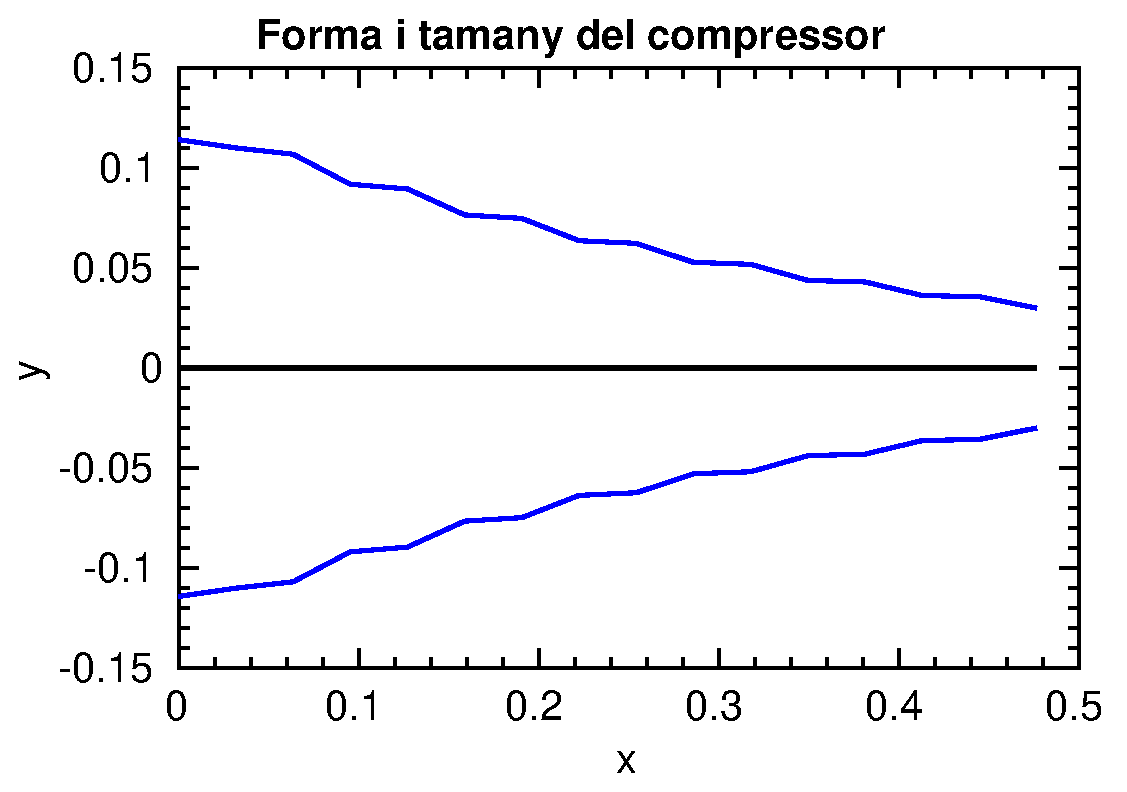
\includegraphics[width=0.8\textwidth]{./code/figures/parametres/compressor_shape.eps}
	\caption{Tamany del compressor}
	\label{shape}
\end{figure}
Realment el compressor no tindria aquesta forma doncs al seu interior la part central aniria creixent de diàmetre. No obstant, l'àrea anular seria la mateixa.
\begin{longtable}[H]{C{5cm} C{2.5cm}}
	\toprule[2pt]
	Longitud del compressor &  \textbf{0.48m} \\ \bottomrule[2pt]
	\caption{Longitud del compressor}
	\label{aleps}
\end{longtable}
Les files de les tres taules següents representen les successives etapes del compressor.
\begin{figure}[H]
	\centering
	\begin{large}\begin{tabular}{|c|c|}
\hline
$h_a$&$h_b$\\\hline
0.11&0.11\\\hline
0.11&0.09\\\hline
0.09&0.08\\\hline
0.07&0.06\\\hline
0.06&0.05\\\hline
0.05&0.04\\\hline
0.04&0.04\\\hline
0.04&0.03\\\hline
\end{tabular}
\end{large}
	\caption{Alçades [m]}
\end{figure}
\begin{figure}[H]
	\centering
	\begin{large}\begin{tabular}{|c|c|c|c|}
\hline
$T_a$&$T_b$&$Tt_a$&$Tt_b$\\\hline
255.32&285.94&288.00&325.35\\\hline
292.68&323.29&325.35&362.70\\\hline
330.03&360.64&362.70&400.05\\\hline
367.38&397.99&400.05&437.40\\\hline
404.73&435.34&437.40&474.75\\\hline
442.08&472.69&474.75&512.10\\\hline
479.43&510.04&512.10&549.45\\\hline
516.78&547.39&549.45&586.80\\\hline
\end{tabular}
\end{large}
	\caption{Temperatures [K]}
\end{figure}
\begin{figure}[H]
	\centering
	\begin{large}\begin{tabular}{|c|c|c|c|}
\hline
$P_a$&$P_b$&$Pt_a$&$Pt_b$\\\hline
64355.72&77586.81&98100.00&121914.41\\\hline
84174.52&125887.48&151509.92&188289.94\\\hline
135309.45&202281.93&233998.54&290803.20\\\hline
215817.24&322736.10&361397.55&449129.15\\\hline
342262.07&512171.65&558158.16&693654.66\\\hline
540449.00&809451.55&862043.82&1071310.54\\\hline
850548.03&1275127.13&1331378.10&1654578.75\\\hline
1335047.53&2003470.97&2056238.46&2555403.65\\\hline
\end{tabular}
\end{large}
	\caption{Pressions [Pa]}
\end{figure}

Després d'analitzar tots els resultats, es creu que donen uns valors lògics que segueixen la mateixa tendència que els mostrats al \textit{Mattingly [Secció 9-4]}. És evident que les hipòtesis introduïdes generen un error. No obstant, són molt útils per obtenir una primera aproximació al disseny un compressor sencer.